
\documentclass[conference]{IEEEtran}
\usepackage[encapsulated]{CJK}
\usepackage{cite}
\usepackage{amsmath,amssymb,amsfonts}
\usepackage{algorithmic}
\usepackage{graphicx}
\usepackage{tabularx}
\usepackage{xcolor}
\usepackage{color}
\begin{document}
\begin{CJK}{UTF8}{bsmi}
\title{Automated Latency Characterization of FAPI and nFAPI under Traffic Loads via an O-RAN SMO rAPP}
\author{
\author{\IEEEauthorblockN{
        Ming-Hong HSU\IEEEauthorrefmark{1}, 
        Ray-Guang Cheng\IEEEauthorrefmark{1},
        Co-author 1\IEEEauthorrefmark{2}
        \\
  }
 \IEEEauthorblockA{\IEEEauthorrefmark{1}
Dept. of Electronic and Computer Engineering, National Taiwan University of Science and Technology, Taiwan
  }
  Email: crg@mail.ntust.edu.tw
}

\IEEEauthorblockA{
Department of Electronic and Computer Engineering, National Taiwan University of Science and Technology\\
Taipei, Taiwan, Republic of China \\
Email: crg@mail.ntust.edu.tw}
}

\maketitle
% 1. 請先各自複製本範本的內容，根據這裡所點出的大綱來寫，無關的內容請勿放入。自己加的內容請用「藍字」，老師改過需要確認會用「紅字」，紅字內容確認無誤的字句請自行改為黑字，有問題改成「藍色」。
% 2. 縮寫字第一次出現前記得要先定義，原則上只有句首第一個字母大寫，請勿誤用！
% 3. 請用國中英文直述句來寫，正確性最重要
% 4. 本範本請先寫System Model、Propose Solution, 以及 Numercial/Experimental Results。Introduction請留到最後
% 5. Introduction僅留下「絕對必要」資訊(沒提到後面就講不下去)即可！
% 6. 使用任何變數前請先「定義」，寫下變數與公式前，請先想清楚，這是「問題」(I/P)、「答案」(O/P)、「推導過程」(Your Algorithm)、還是「範例」(Example)
% 問題與答案放在System Model，
% 推導過程放在Analytical Model，
% 範例放在Numercial Results

Abstract Section (before Introduction)
Add a clear placeholder for an abstract:

Purpose: Briefly summarize the problem, method, results, and contribution.

Word count: typically 150–250 words.

Keywords: list 3–6 keywords.

\section{Introduction}
\subsection{Introduction}
{\bf Purpose:} To explain {\bf what} the paper is about, {\bf why} the problem matters, and {\bf what} the others authors have done to address it.

Typical content:
\begin{itemize}
\item Background and motivation
\item Problem statement
\item Goals of the paper
\item Contributions (what’s new or important)
\item High-level overview of the approach or results
\end{itemize}

Example phrases:
\begin{itemize}
\item “In recent years, …”
\item “This paper addresses the problem of …”
\item “Our main contributions are …”
\end{itemize}



\subsection{Related Works}
{\bf Purpose:} To show how your work fits into the existing body of knowledge, and how it differs from or improves upon previous work.

Typical content:
\begin{itemize}
\item Summary of key prior research
\item Strengths and limitations of existing approaches
\item Comparison to your approach
\item Justification for why a new approach is needed
\end{itemize}

Example phrases:
\begin{itemize}
\item “Several studies have explored …”
\item “Unlike [Author], we propose …”
\item “Prior work has not considered …”
\end{itemize}

% Background Knowledge directly related to Your Thesis Title

% Related Work

% Contribution: The last TWO paragraphs of your paper.
The main contributions of this paper are summarized as follows.
\begin{itemize}
\item Contribution 1.
\item Contribution 2. 
\item Contribution 3. 
\end{itemize}

% The rest of the paper is organized as follows. Section II defines the system model/architecture considered in this paper. The proposed analytical model/method is given in Section III. Section IV shows the numerical results. Concluding remarks are given in Section VI.

\section{System Model/Architecture}

% To all 2nd Yr students,
% You have to start writing your thesis now. I already show you the template.
% Please focus on Problem & Solution
% Problem (題目) Sec. II System Model
% Solution (答案) Sec. III Proposed Method
% Show me your system architecture/block diagram, flowchart and clearly define the I/Ps and O/Ps your compunents. (先把系統架構圖、流程圖畫清楚，解釋清楚你怎麼做)

% \begin{figure}
%     \centering
%     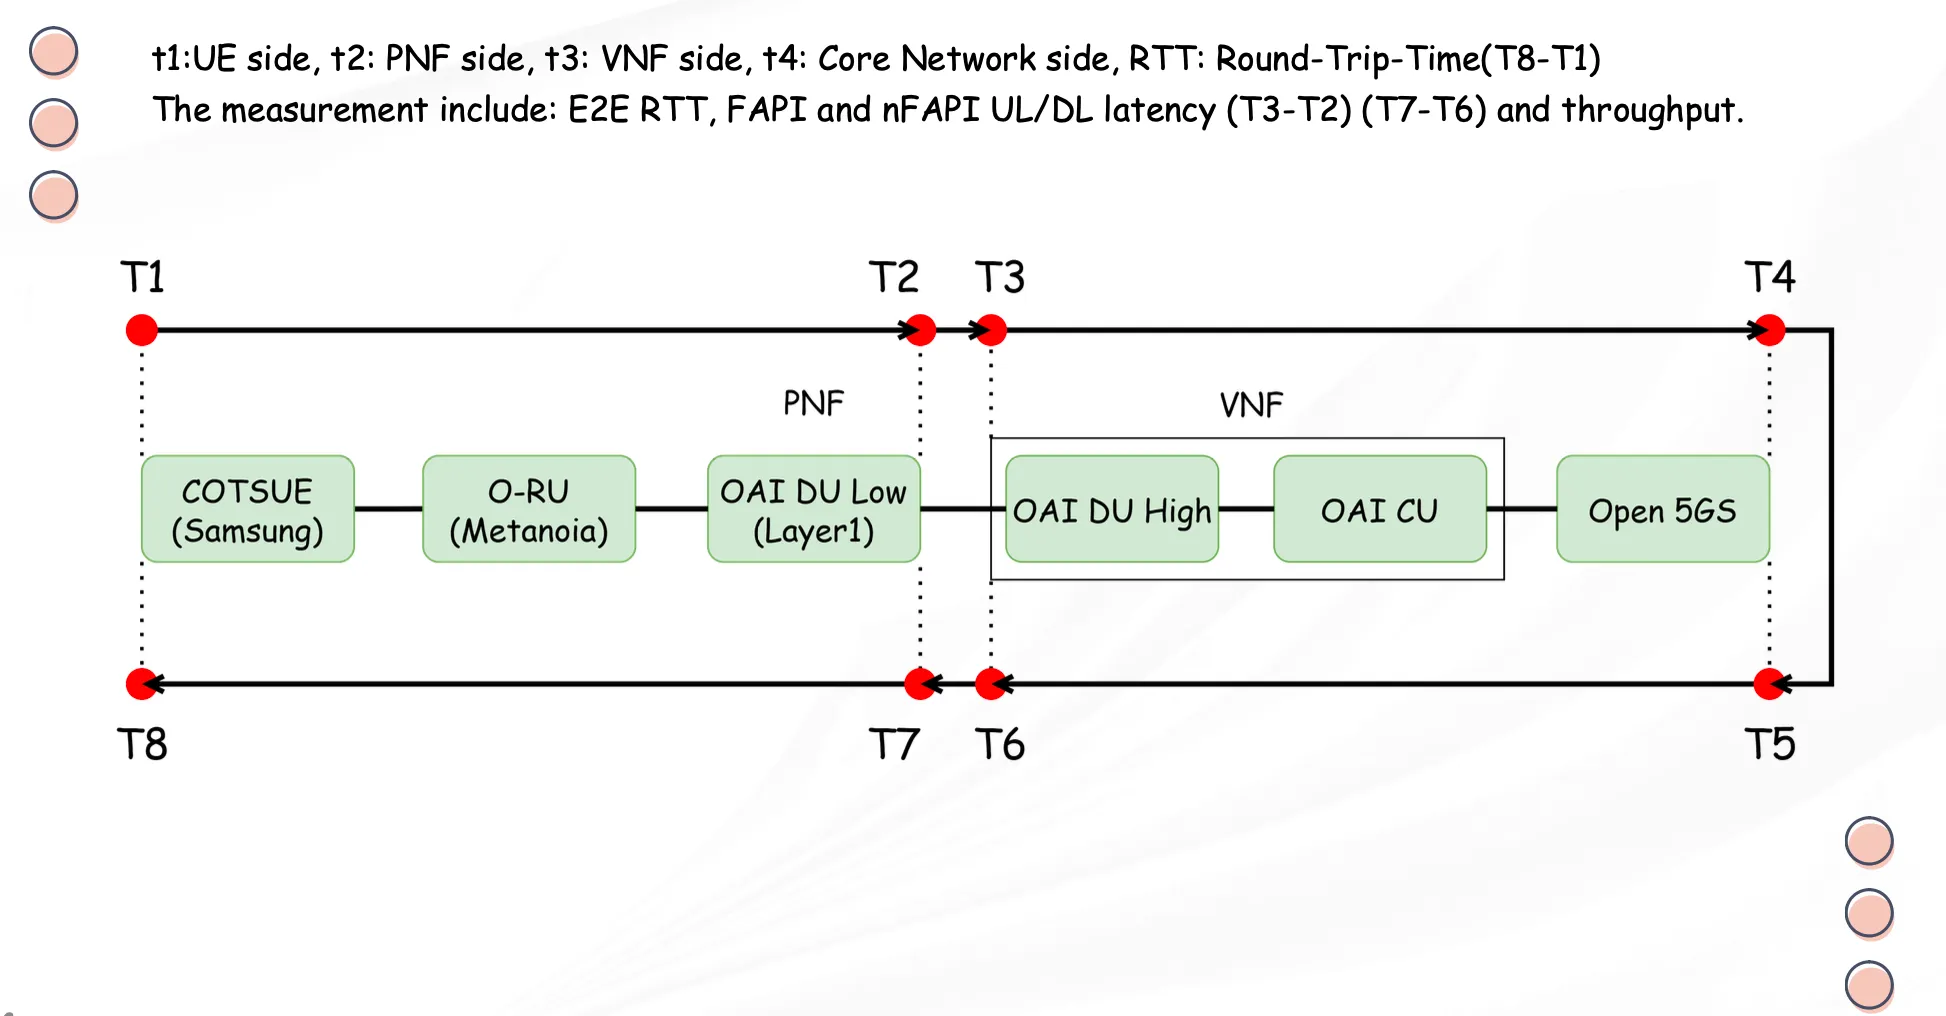
\includegraphics[width=0.5\linewidth]{image.png}
%     \caption{End-to-End measurement}
%     \label{fig:placeholder}
% \end{figure}

% Figure~\ref{fig:Fig1} shows the system model/architecture considered in this paper.
% (Draw a figure showing the key components and their relationship in the system model. It may consist the I/P and O/P parameters of your system or the major components showing your contributions.) 
% \begin{figure}[h]
%   \centerline{\includegraphics[width=1\columnwidth]{root/fig1_v5.png}}
%   \caption{Timing diagram of the system model considered in this paper.}
%   \label{fig:Fig1}

% \end{figure}
% 用一個大括號{} 將這個區間內的文字都設定成藍色字體
{\color{blue}

The following assumptions were made in this paper.
\begin{itemize}
\item 5G O-RAN架構下End-to-End的自動化性能評估挑戰
\item O-RAN SMO智能管理需求
\item FAPI 與 NFAPI的比較研究分析
\end{itemize}



隨著5G技術的發展和O-RAN聯盟推動開放式架構，\textbf{FAPI (Functional Application Platform Interface)} 和 \textbf{nFAPI (network FAPI)} 作為關鍵的拆分介面標準，其性能差異對實際部署具有重大影響。電信運營商和設備供應商需要客觀資料來選擇合適的功能分割架構，以平衡成本與性能。以目前實驗室合作的計畫案為例，義傳科技等專門從事RU開發的公司在整合DU LOW和RU時，需要依據可靠數據選擇適合的分割點（\textbf{split 6}）架構。

\vspace{1em}

目前學術界與業界缺乏End-to-End環境下FAPI與nFAPI架構性能差異的系統性測量工具，特別是缺乏自動化的\textbf{throughput}、\textbf{latency}及\textbf{CPU資源使用率}綜合呈現方案。現有測試方法多依賴人工干預和簡單指標測量，無法提供全面且可重現的性能比較結果。

\vspace{1em}

在O-RAN架構中，\textbf{Service Management and Orchestration (SMO)} 框架提供統一的管理服務，\textbf{Non-RT RIC}支援非即時的無線電資源管理和策略優化。而現有的rApp主要聚焦於特定功能（如能源管理、網路切片），但缺乏專門針對End-to-End性能自動化測量的通用解決方案。



% \section{Proposed Method}
% \section{Numerical/Simulation/Experimental Results}
% Computer simulations/Experiments were conducted to verify xxx (the effectiveness of the proposed analytical model). 
% In the following figures, each point represented the average value of $10^5$ samples. In each sample, we collect the statistics of xxx. Symbols and lines were used to show the simulation and analytical results, respectively. 

\section{研究方法}

\subsection{第一階段：End-to-End自動化測量rApp設計與開發}
\textbf{rApp架構設計}
\begin{itemize}
    \item 在O-RAN SMO框架中開發專門的rApp，支援End-to-End環境下的自動化性能測量
    \item 整合測試該環境最高throughput、該環境latency、可靠性、CPU使用率等多維度指標的報告生成
    \item 設計可配置的測量參數和測試場景，支援小流量到大流量的自動化測試
\end{itemize}

\textbf{實現}
\begin{itemize}
    \item 利用O-RAN SMO rApp的互動機制，實現對底層網路功能的環境自動化建置（可基於Joe's rAPP去延伸，搭配Summer's rapp去整合）
\end{itemize}

\subsection{第二階段：FAPI與nFAPI架構下的比較測試}
\begin{itemize}
    \item 基於OpenAirInterface的實驗平台
    \item 運用EURECOM實習期間開發的nFAPI和實驗室既有的FAPI實作經驗
    \item 建立統一的測試環境，確保兩種架構測試條件的一致性
    \item 實現自動化測試腳本（可建置於SMO rApp），支援可重複的實驗流程
\end{itemize}

\textbf{系統性性能測量}
\begin{itemize}
    \item 運用開發的rApp分別在FAPI和nFAPI架構下進行End-to-End性能測量
    \item 執行小流量到大流量條件下的延遲、吞吐量比較測試
    \item 分析兩種架構在不同負載下的系統資源使用效率
\end{itemize}

\subsection{第三階段：OpenAirInterface優化與驗證}
\textbf{FH優化}
\begin{itemize}
    \item [暫定] 基於發現的OAI前傳接口錯誤封包處理問題，設計跳過機制的優化方案
    \item [暫定] 實作優化方案並驗證其對系統流量處理能力的提升效果
    \item [暫定] 評估優化方案在不同架構下的適用性和穩定性
\end{itemize}

\begin{quote}
目前已實作且得到Robert的認可方法合理，但只能從結果提出證據驗證有效，且無法100\%驗證完全根本解決問題，算是一種暫時性解法。
\end{quote}

% \textbf{性能改進驗證}
% \begin{itemize}
%     \item 驗證優化方案對FAPI和nFAPI架構性能影響的差異性
% \end{itemize}

\section{研究貢獻}

\begin{itemize}
    \item 新穎的End-to-End自動化測量rApp
    \item 通用性能測量解決方案
    \item 開發首個專門針對End-to-End性能自動化測量的O-RAN rApp
    \item 提供標準化的測量框架，支援不同廠商和部署環境的通用性應用與參考報告
    \item RU支援Metanoia, pegatron, liteon
    \item UE支援root Android
    \item 實現throughput、latency、資源使用率等多維度指標的報告
\end{itemize}

\begin{quote}
進階功能展望：
\begin{itemize}
    \item 更花俏的功能？
    \item 套用LLM API提供報告之摘要
    \item 提供可視化的性能分析UI 報告
\end{itemize}
\end{quote}


\textbf{FAPI vs nFAPI性能數據集}
\begin{itemize}
    \item 全面的比較分析結果
    \item 基於實際測量提供FAPI與nFAPI在各種流量條件下的延遲、吞吐量比較數據
    \item 建立包含系統資源使用效率、記憶體使用率的完整性能數據集
    \item 提供不同硬體配置和網路條件下的架構選擇決策模型
    \item 提出觀點：NFAPI將DU分散在兩個server上跑真的會分擔CPU效能嗎？還是不會？
\end{itemize}

\textbf{OpenAirInterface平台優化方案}
\begin{itemize}
    \item FH改進
    \item 提出針對OAI錯誤封包處理的跳過機制優化方案
    \item NFAPI mode修復
    \item 於法國EURECOM與工程師合作參與NFAPI修復開發計畫，並貢獻開源社群，推動OpenAirInterface平台的持續改進
\end{itemize}

\section{學術與產業應用價值}
\textbf{學術貢獻}
\begin{itemize}
    \item 填補O-RAN架構下End-to-End自動化性能測量的研究空白
    \item 提供系統性的FAPI與nFAPI比較分析方法
    \item 推動5G功能分割標準化和優化的學術研究發展
\end{itemize}

\textbf{產業應用價值}
\begin{itemize}
    \item 為電信運營商和設備供應商提供架構選擇的客觀決策依據
    \item 支援O-RAN生態系統的互操作性測試和驗證流程
    \item 促進開源5G軟體平台的性能改進和廣泛採用
\end{itemize}

\section*{本研究優勢}
\begin{itemize}
    \item 創新性：提出End-to-End自動化測量rApp的新概念，填補現有研究空白
    \item 實用性：基於實際的OpenAirInterface實作經驗和業界真實需求
    \item 系統性：從工具開發到架構比較，再到平台優化的完整研究流程
    \item 貢獻明確：同時具備學術價值和產業應用潛力的具體成果
    \item 技術可行性：建立在已有的實作基礎和成熟的O-RAN標準之上
\end{itemize}
}


%很多同學無法討論的原因是因為花了很多時間畫圖，但是圖畫錯。
%圖畫錯的原因是在畫圖前沒有先思考過，依據手邊的資料打算畫出怎麼樣的圖？這些圖是否能呈現想表達的意義？
%所以在規劃的時候應該是從目標回頭來看:
%告訴大家貢獻是什麼？
%預期從資料分析結果的哪些現象可以證明你的貢獻？
%想觀察什麼現象？
%這些現象從什麼的圖可看出？
%如何畫出這樣的圖？需要哪些資料？
% XXX scenarios were investigated. Scenario I was designed to demonstrate/verify the accuracy/effectiveness of Contribution 1.

% For each contribution, tell us
% HOW do you design experiments to demonstrate your contribution 
% WHY your results can support your contribution
% \subsection{Contribution 1}
% Fig. 1.1: Purpose
%     X axis: 
%     Y axis:
% \subsection{Contribution 2}
% Fig. 2.1: 
%     X axis: 
%     Y axis:
% \subsection{Contribution 3}
% Fig. 3.1: 
%     X axis: 
%     Y axis:
% \begin{thebibliography}{00}
% \bibitem{b1} 
\end{thebibliography}
\end{CJK}
\end{document}

